\documentclass {report}
%Bibliotēkas
\usepackage[utf8]{inputenc}
\usepackage{hyperref}
\usepackage{url}
\usepackage{polyglossia}
\usepackage{graphicx}
\usepackage{fancyvrb}
\usepackage[siunitx,europeanresistors,americaninductors]{circuitikz}
\usepackage{tikz}
\usepackage{pgfplots}
\usepackage{geometry}
\usepackage{float}
%Papīra formāts
\geometry{
 a4paper,
 total={170mm,257mm},
 left=20mm,
 top=20mm
 }
%Grafiku režģlīnijas
\pgfplotsset{minor grid style={dashed,red}}
\pgfplotsset{major grid style={dotted,green!50!black}}
%Iebūvēto komandu/var pārsaukšana
\renewcommand{\chaptername}{Nodaļa}
\renewcommand{\tablename}{Tabula}
\renewcommand{\figurename}{Attēls}
\renewcommand{\bibname}{Atsauces}
%Titullapas elementi
\title{Vienkāršu elektrisku shēmu modelēšana}
\author{Dāvis Muižnieks}
\date{2019. gada 13. marts}
%Dokumenta sākums
\begin{document}

\maketitle
\chapter{Teorētiskā daļa}
\section{Ķēdes aprēķins}
Veicot elektriskās ķēdes sprieguma dalītāja aprēķinus teorētiski, tika iegūti dati, kas redzami tabulā \ref{tab:1st}.
%Tabulas piemērs
\begin{table}[!h]
    \centering
    \small\addtolength{\tabcolsep}{10pt}
    \begin{tabular}{|c|c|}
        \hline \multicolumn{2}{|c|}{Tabula:} \\
        \hline
        R1 & 9Ω\\
        \hline
        R2 & 8Ω\\
        \hline
        V1 & 38,7V\\
        \hline
        $U_{R1}$ & 20,488V\\
        \hline
        $U_{R2}$ & 18,212V\\
        \hline
    \end{tabular}
    \caption{Aprēķinātās vērtības}
    \label{tab:1st}
\end{table}
%Teksta formatēšanas piemērs
\textbf{\textit{Aprēķina gaita redzama zemāk.}} Aprēķinu veikšanai izmantota informācija no papildus materiāliem, \cite{Source:1st}.
\\[0.5cm]
{\large\textbf{Apliecības numurs: 171RMC100}\\
* $U=V_{1}$ = 38.7V\\
* R$_{1}$ = 9\\
* R$_{2}$ = 8\\
* I = \( \frac{V}{R} \) = \( \frac{38.7}{17}\) = 2.276 A\\
* V$_{R1}$ = I*R = 2.276*9 = 20.488 V\\
* V$_{R2}$ = I*R = 2.276*8 = 18.212 V\\
* V$_{total}$ = V$_{1}$ + V$_{2}$ = 20.488 + 18.212 = 38.7 V\\
\par}
%Shēmas zīmēšanas piemērs
\begin{center}
\begin{circuitikz} [scale=1.3, every node/.style={transform shape}]
    \draw
    (0,0) to[R=$R_1$, *-*] (4,0)
    (4,0) to[R=$R_2$] (4,-2)
    (0,-2) to[short] (4,-2)
    (0,0) to[battery1=$V_1$, *-*] (0,-2)
    ;
\end{circuitikz} 
%Grafika zīmēšanas piemērs
\begin{tikzpicture}
  \begin{axis}[
    grid=both,
    minor tick num=1,
    xlabel=$U_{R2}$,
    ylabel={$f(R2) = U/R$}]
        \addplot[mesh,scatter,samples=10,domain=0:18.212] {x/8};
    \end{axis}
\end{tikzpicture}
\end{center}
Shēma un grafiks izveidots ar LaTeX iekļauto bibliotēku palīdzību \cite{Source:2nd} \cite{Source:3rd}.
%Jauna nodaļa
\chapter{Praktiskā daļa}
\section{Darbs ar gEDA programmām}
\subsection{Darbs ar gschem}
    \begin{figure}[!h]
        \centering
            \rotatebox{-90}{\includegraphics[width=15cm,height=15cm,keepaspectratio]{pictures/01.ps}}
        \caption{Iegūtā shēma ar gschem}
        \label{fig:1st}
    \end{figure}
\indent Programmā \textit{gschem} tika sastādīta shēma (skat. attēlu \ref{fig:1st}), atbilstoši veiktajam teorētiskajam aprēķinam (skat. nodaļu Teorētiskā daļa). Katram elementam tika pievienotas atbilstošās vērtības, kuras skatāmas tabulā \ref{tab:1st}. Ar šīs programmas palīdzību tika izveidots ".ps" attēla fails.
\pagebreak

\subsection{Darbs ar gnetlist}
\VerbatimInput{text-based/01.net} 
\hrule \relax
\indent Ar gnetlist programmu iespējams iegūt netlist failu "*.net", kas satur informāciju par elementu vērtībām, savienojumiem un nosaukumiem no shēmu faila "*.sch"

\subsection{Darbs ar ngspice}
\indent Pēc netlist faila pārbaudes ar komandu "cat", to var izmantot simulācijai ar programmu "ngspice". \\
\indent \textbf{Attēlā \ref{fig:2nd}} ir attēlots pārejas process (tran) simulācija \textbf{1. signālu savienojumam} no 0 līdz 5 sekundēm ar soli 1 sekunde. \\
\indent \textbf{Attēlā \ref{fig:3rd}} ir attēlots pārejas process (tran) simulācija \textbf{2. signālu savienojumam} no 0 līdz 5 sekundēm ar soli 1 sekunde.

\begin{figure}[!h]
    \centering
        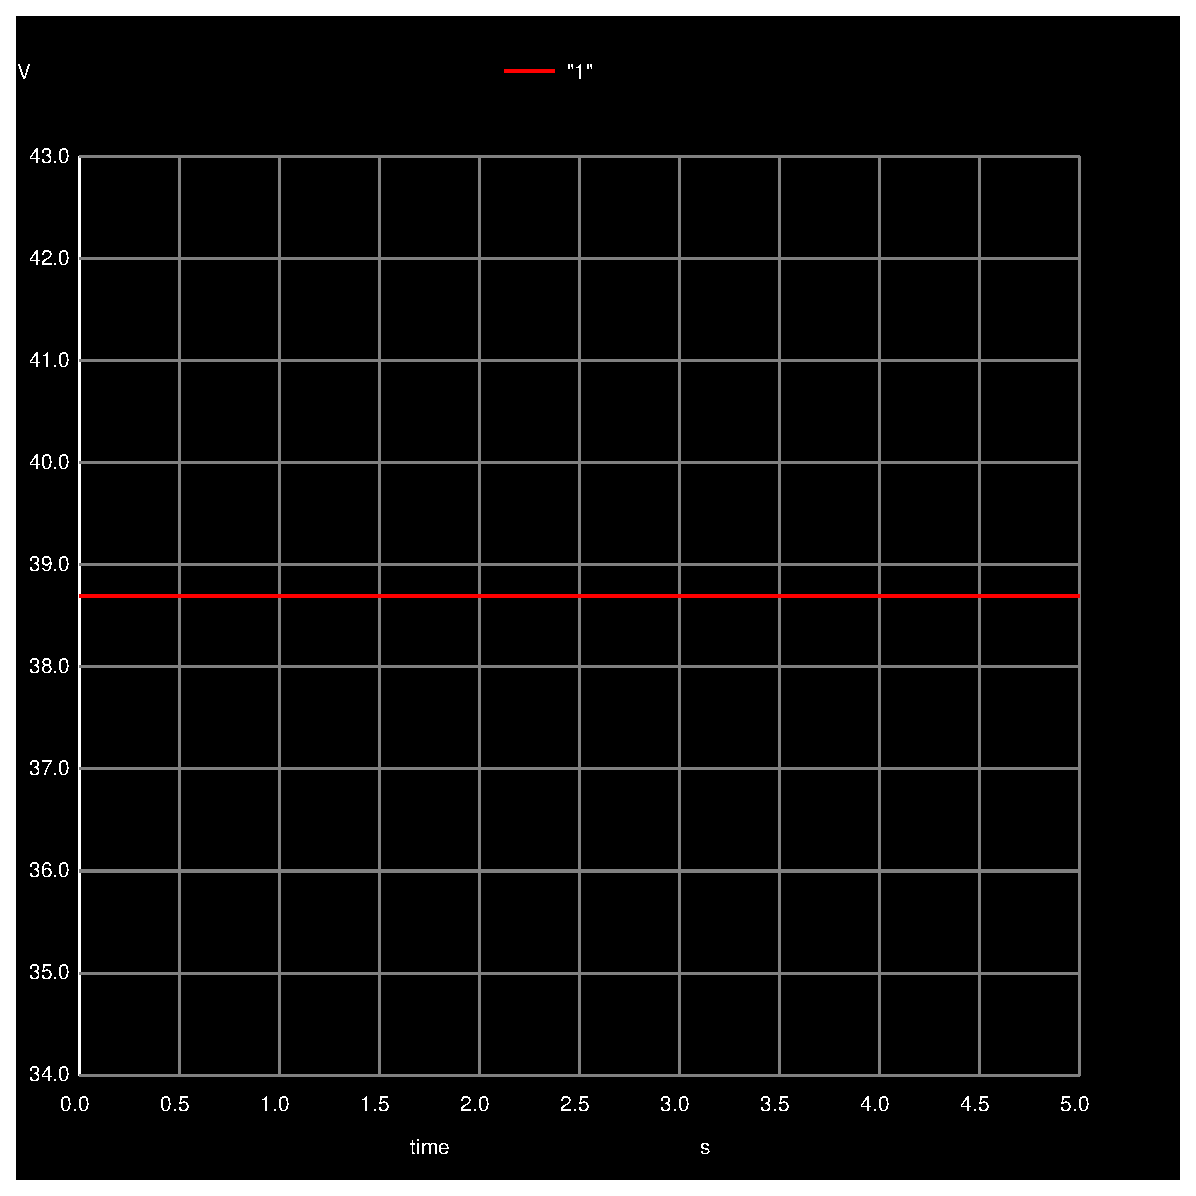
\includegraphics[width=16cm,height=16cm,keepaspectratio]{pictures/011.ps}
    \caption{Simulācija 1. signālu savienojumam}
    \label{fig:2nd}
\end{figure}

\pagebreak

\begin{figure}[!h]
    \centering
        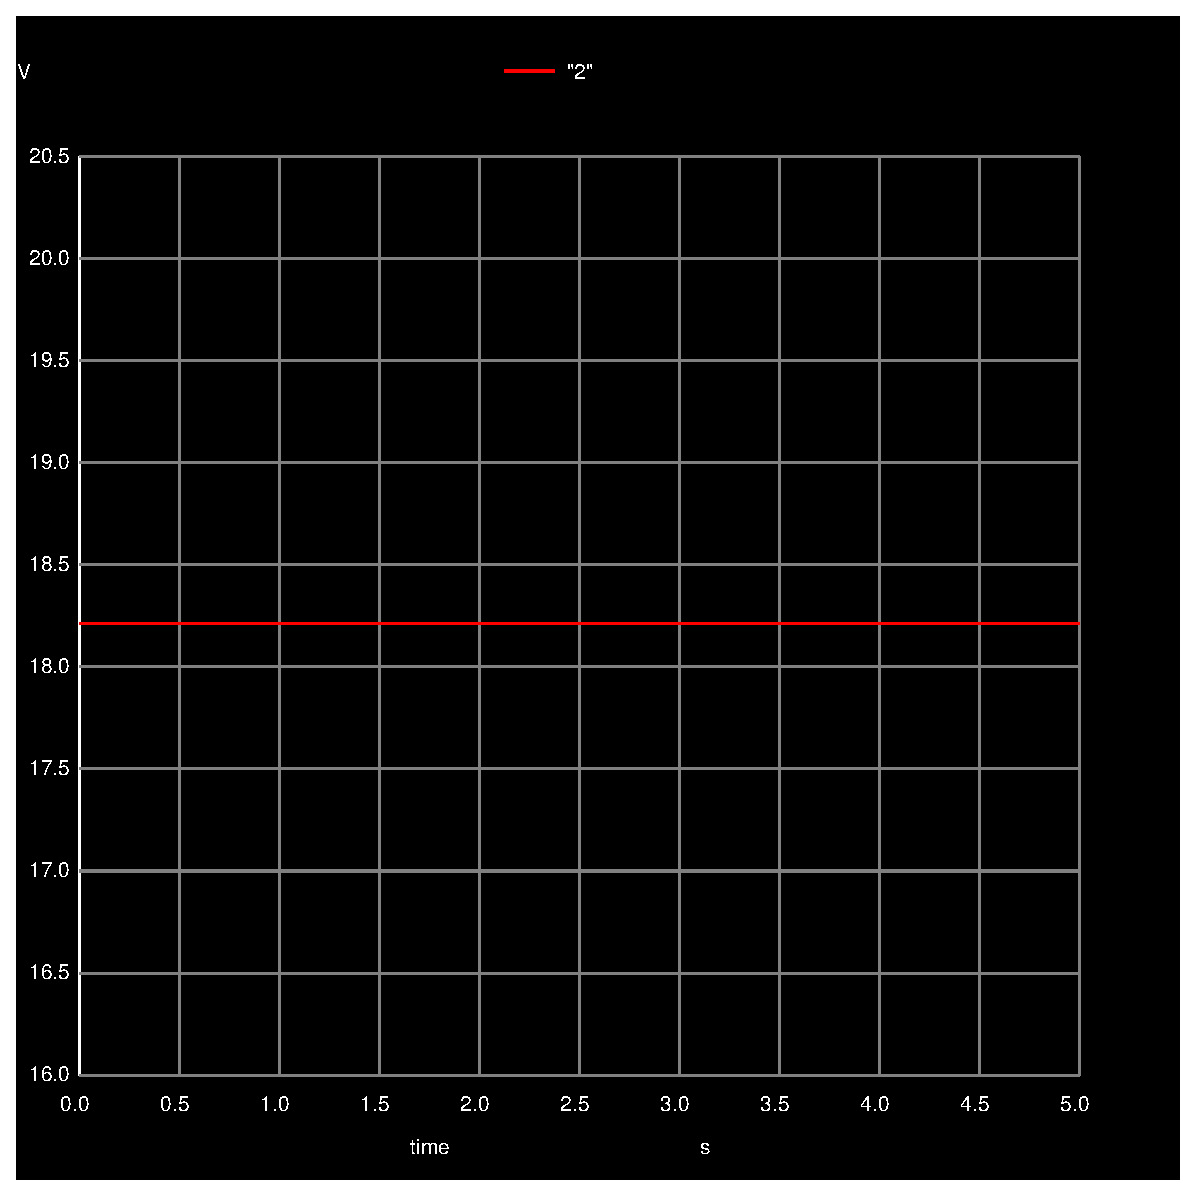
\includegraphics[width=16cm,height=16cm,keepaspectratio]{pictures/012.ps}
    \caption{Simulācija 2. signālu savienojumam}
    \label{fig:3rd}
\end{figure}
\newpage

\section{Darbs ar QUCS programmām}
QUCS - shēmu simulāciju programma. Ar to iespējams ērti izvēlēties komponentes un veidot savienojumus. Vērtības ir izvēlētas atbilstoši teorētiskajiem aprēķiniem, izņemot R2.
\subsection{Pricipālā shēma:}
\VerbatimInput{schemes/02.sch}
\pagebreak

\subsection{Līdzstrāvas simulācijas grafiks:}
\begin{figure}[h]
    \centering
        \rotatebox{-90}{\includegraphics[trim={1.2cm 1cm 16cm 21cm},clip]{pictures/02_scheme.ps}} %% augša, kreisā puse, apakša, labā puse
    \caption{Līdzstrāvas režīma simulācija}
    \label{fig:4th}
\end{figure}
    
\indent Izveidota shēma elementāra līdzstrāvas režīma simulācijai ar simulācijas komponenti "Parameter sweep". (skat. attēlu \ref{fig:4th})\\
R2 vietā tiek izmantots mainīgais "x", kas norādīts arī "Parameter sweep" komponentē, kura tiks izmantota sweep simulācijas grafika radīšanai. \\ Veicot simulēšanu, x vērtība (jeb R2) maiņa notiks lineāri, sākot no vērtības 5Ω līdz 50Ω vienpadsmit punktos (sākuma punkts + 10 sekojošie punkti), kuros tiek pārrēķināti visi ķēdes parametri (strāvas un spriegumi) saistībā ar R2 maiņu.\\

\subsection{Sweep simulācijas līdzstrāvas grafiks un tabula:}
\begin{figure}[h]
    \centering
        \rotatebox{-90}{\includegraphics[trim={1cm 1cm 14cm 24cm},clip]{pictures/02.ps}} %% augša, kreisā puse, apakša, labā puse
    \caption{Simulācijas grafiks un tabula}
    \label{fig:5th}
\end{figure}

\indent Iepriekš veiktās simulācijas rezultātā, iegūstam grafiku un tabulu (skat. attēlu \ref{fig:5th}), kuros uzrādīti iegūtie dati 11 punktos, kurus var izmantot shēmas diagrammu (*.dpl) darba formā. Izvēloties Dekarta koordinātu sistēmas diagrammu komponenti un punktu "izeja", iegūstam grafiku, kas rāda funkcionālu sakarību starp mainīgo R2 vērtību un spriegumu uz tā - UR2. \\ \indent Uz darba formas atrodas arī tabula, kurā attēlota strāvu "V1.I" (plūst caur sprieguma avotu V1) un el. ķēdes punkta "Izeja" attiecība.
%Atsauces
\begin{thebibliography}{9}
\bibitem{Source:1st}
Andrejs Strauts, Elektrotehnikas teorētiskie pamati: lekciju konspekts. Rīga: RTU, 2007.
\bibitem{Source:2nd}
Vairāki elementi no dažādiem autoriem;  \url{https://tex.stackexchange.com/}
\bibitem{Source:3rd}
Overleaf learning database; \url{https://www.overleaf.com/learn/latex/Pgfplots_package}
\end{thebibliography}
%Dokumenta beigas
\end{document}
